\chapter{Anhang}
\section{Artikel \cite{paper}}
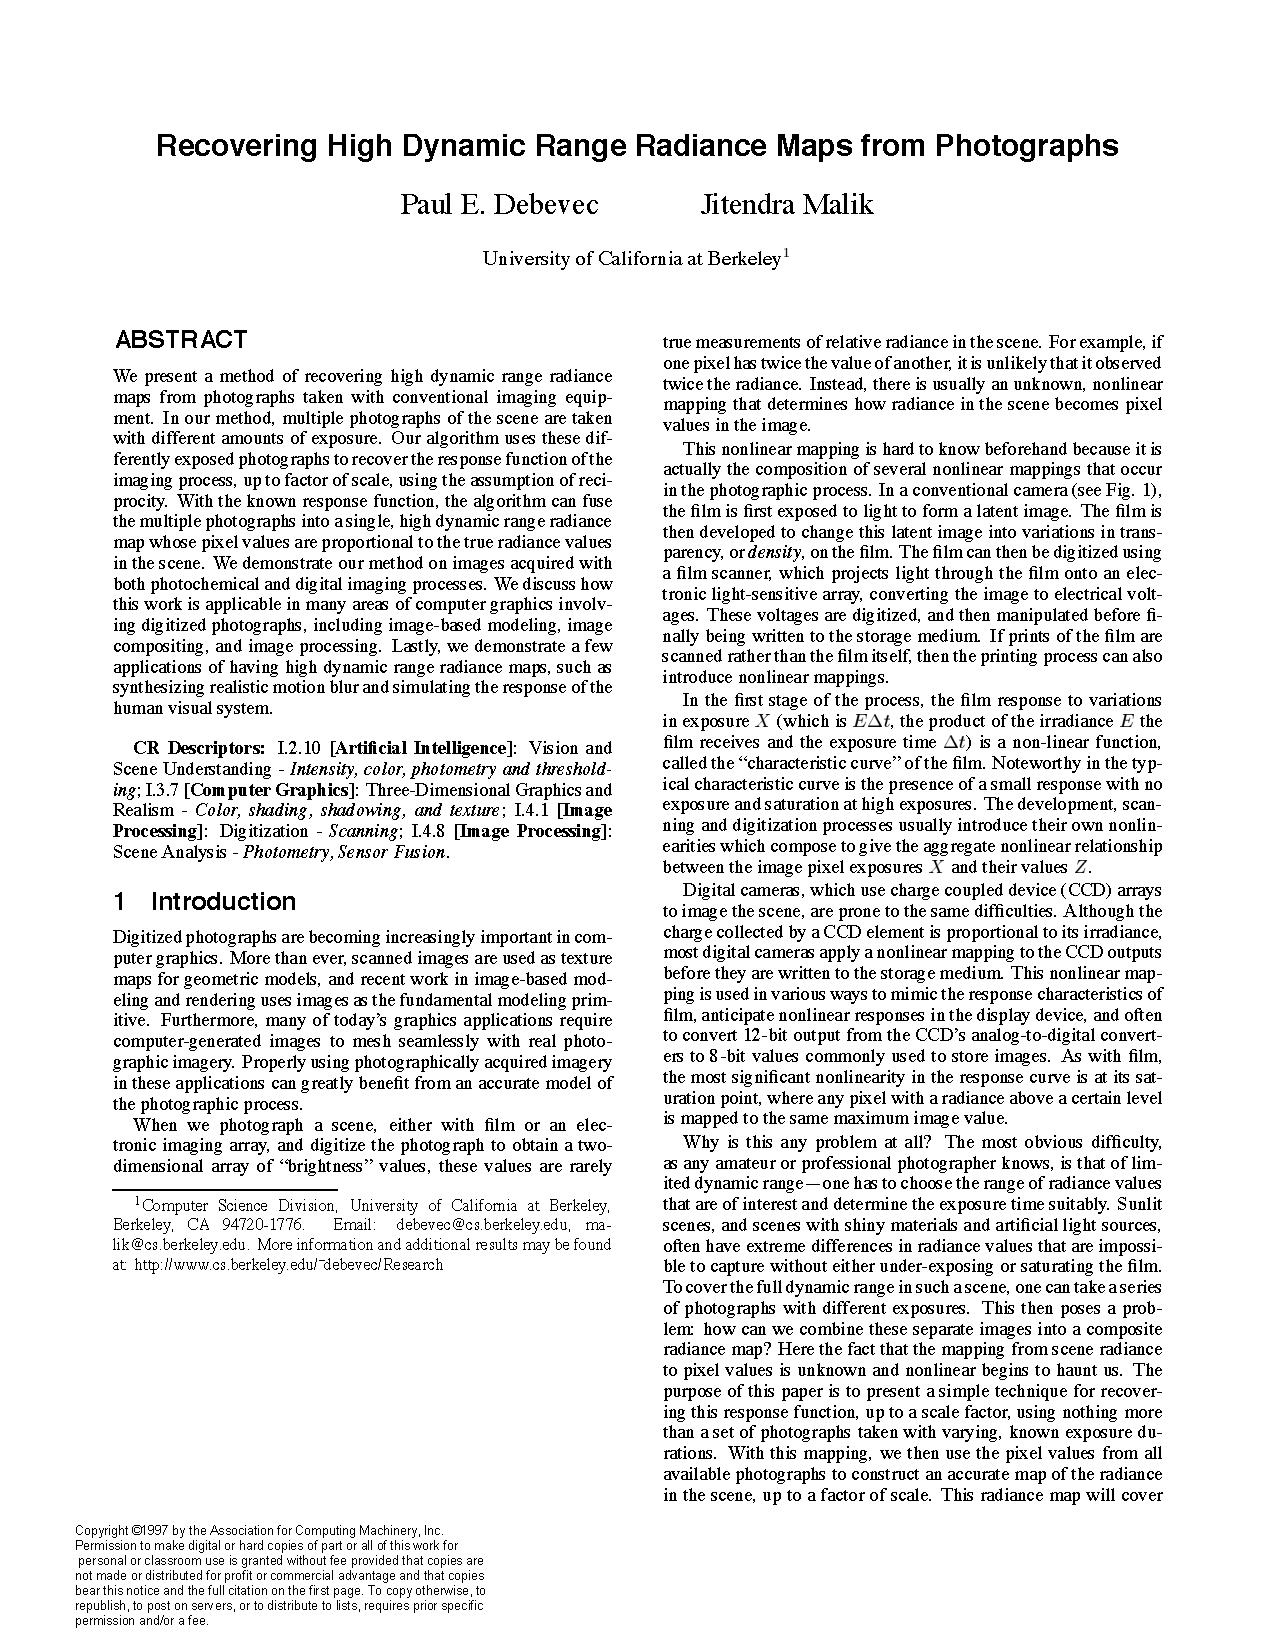
\includepdf[pagecommand={},pages=-,scale=0.8]{content/attachment/00_Artikel.pdf} 
\section{Verwendete Algorithmen}

\subsection{MTB-Algorithmus, vgl. \cite[S.9 f]{Ward03fast}}
\label{subsec:MTB}
Dem \gls{MTB} Verfahren (vgl. \cite{Ward03fast}) wird eine Serie von $N$ Bildern als Eingabe geliefert. Diese werden zunächst in ein Grauwert-Bild umgerechnet. Aus diesen Bildern wird der Algorithmus dann ausgehend von einem gewähltem Bild $N-1$ Offsets $(x,y)$ ausgeben, sodass die Bilder exakt übereinander gelegt werden können (vgl. \cite[S. 123f]{Reinhard}). Eine Alignierung von rotierten Bildern ist somit mit diesem Verfahren nicht möglich. 

Das Verfahren arbeitet dabei im Gegensatz zu vielen konventionellen Algorithmen nicht mit Kanten-Detektion im Bild um die Alignierung durchzuführen, da diese sehr anfällig auf unterschiedliche Belichtungswerte in Bildern sind. Es kommt hingegen ein Schwellwert-Verfahren auf einer Bilderpyramide zum Einsatz, dass dann mit schnellen Bit-Operationen die Verschiebung der Bilder berechnet (vgl. \cite{Ward03fast}). Der Code dazu befindet sich im Anhang (siehe \autoref{lst:MTB:core}).

\begin{Listing}[H]
\label{lst:MTB:helpers}
\begin{lstlisting}[language=c]
/** Subsample the image img by a factor of two in each dimension 
 *  and put the result into a newly allocated image img_ret.*/
ImageShrink2(const Image *img, Image *img_ret)

/** Allocate and compute the threshold bitmap tb and the exclusion bitmap eb for the image img. 
 *  (The threshold and tolerance to use are included in the Image struct.)*/
ComputeBitmaps(const Image *img, Bitmap *tb, Bitmap *eb)

/** Shift a bitmap by (xo,yo) and put the result into the preallocated 
 *  bitmap bm_ret, clearing exposed border areas to zero. */
BitmapShift(const Bitmap *bm, int xo, int yo, Bitmap *bm_ret)

/** Compute the exclusive-or of bm1 and bm2 and put the result into bm_ret. */
BitmapXOR(const Bitmap *bm1, const Bitmap *bm2, Bitmap *bm_ret)

/** Compute the sum of all 1 bits in the bitmap. */
BitmapTotal(const Bitmap *bm)
\end{lstlisting}
\caption{Hilfsfunktionen in C Funktion zur Berechnung der Alignierung}

\end{Listing}

\begin{Listing}[H]
\label{lst:MTB:core}
\begin{lstlisting}[language=c]
/** Computes the shift between two images img1 and img2.**/
GetExpShift(const Image *img1, const Image *img2, int shift_bits, int shift_ret[2])
{
    int min_err;
    int cur_shift[2]; Bitmap tb1, tb2; Bitmap eb1, eb2;
    int i, j;
    if (shift_bits > 0) {
        Image sml_img1, sml_img2;
        ImageShrink2(img1, &sml_img1);
        ImageShrink2(img2, &sml_img2);
        GetExpShift(&sml_img1, &sml_img2, shift_bits-1, cur_shift); ImageFree(&sml_img1);
        ImageFree(&sml_img2);
        cur_shift[0] *= 2;
        cur_shift[1] *= 2;
    } else
    cur_shift[0] = cur_shift[1] = 0;
    ComputeBitmaps(img1, &tb1, &eb1);
    ComputeBitmaps(img2, &tb2, &eb2);
    min_err = img1->xres * img1->yres;
    for (i = -1; i < = 1; i++)
    for (j = -1; j <= 1; j++) {
        int xs = cur_shift[0] + i;
        int ys = cur_shift[1] + j;
        Bitmap shifted_tb2;
        Bitmap shifted_eb2;
        Bitmap diff_b;
        int err;
        BitmapNew(img1->xres, img1->yres, &shifted_tb2); BitmapNew(img1->xres, img1->yres, &shifted_eb2); BitmapNew(img1->xres, img1->yres, &diff_b); BitmapShift(&tb2, xs, ys, &shifted_tb2); BitmapShift(&eb2, xs, ys, &shifted_eb2); BitmapXOR(&tb1, &shifted_tb2, &diff_b); BitmapAND(&diff_b, &eb1, &diff_b); BitmapAND(&diff_b, &shifted_eb2, &diff_b);
        err = BitmapTotal(&diff_b);
        if (err < min_err) {
            shift_ret[0] = xs;
            shift_ret[1] = ys;
            min_err = err;
        }
        BitmapFree(&shifted_tb2);
        BitmapFree(&shifted_eb2);
    }
    BitmapFree(&tb1); BitmapFree(&eb1);
    BitmapFree(&tb2); BitmapFree(&eb2);
}
\end{lstlisting}
\caption{Rekursive C Funktion zur Berechnung der notwendigen Verschiebung zwischen den Bildern um diese zu alignieren}
\end{Listing}

\subsection{LU-Zerlegung}
\begin{Algorithmus}[H]
\caption{Lösen von $A\cdot x = b$ mittels LU-Zerlegung (A ist pentadiagonal)}
\label{alg:LU}
\begin{algorithmic}
\Function{LUDecomposition}{$A$}
	\If{!\Call{isPentadiagonale}{$A$}}
	    \State \Return error
	\EndIf
    \State $m_0 \gets A_{0,0}$, $\qquad r_0 \gets A_{0,1}$, $\qquad l_0 \gets A_{1,0}/m_0$, $ \qquad m_1 \gets A_{1,1}- l_1r_0$
    \ForAll{$i \in [2,n]$}
        \State $p_i \gets A_{i-2,i}$
        \State $k_i \gets A_{i,i-2}/m_{i-2}$
        \State $r_{i-1} \gets A_{i-1,i} - l_{i-1}  p_{i-2}$
        \State $m_i \gets A_{i,i} - k_i p_{i-2} - l_i  r_{i-1}$
        \State $l_i \gets (A_{i,i-1}-k_i r_{i-2})/m_{i-1}$
    \EndFor
    \State $L \gets $\Call{generateL}{$l$, $k$}         \Comment{Generiert die Matrix L und U }
    \State $U \gets $\Call{generateU}{$m$, $r$, $p$}    \Comment{nach obigem Schema (siehe \autoref{eq:lu:structure})}
    \State \Return [L, U]
\EndFunction

\Function{forwardElimination}{b,L}
        \State $y_0 \gets b_0$
        \State $y_1 \gets b_1 - L_{1,0} y_0$
        \For{$i = 2 \mbox{ to } size(b)$}
            \State $y_i \gets b_i - L_{i,i-2} y_{i-2} - L_{i,i-1} y_{i-1}$
        \EndFor
        \Return $y$
\EndFunction


\Function{backwardSubstitution}{U,y}
        \State $x_{n-1} \gets y_{n-1}/U_{n-1,n-2}$
        \State $x_{n-2} \gets (y_{n-2} - U_{n-2,n-1} x_{n-1})/U_{n-2,n-2}$
        \State $y_1 \gets b_1 - L_{1,0} y_0$
        \For{$i = size(b)-3 \mbox{ to } 0$}
            \State $x_i \gets (U_{i,i+1} x_{i+1}- U_{i,i+2} x_{i+2} - y_i) / U_{i,i}$
        \EndFor
        \Return $x$
\EndFunction




\Function{Solve}{$A$, $b$}
	\If{\Call{size}{$A$} != \Call{size}{b}}
	    \State \Return error
	\EndIf
	\State [L,U] = \Call{LUDecomposition}{A};

    \State $y \gets $\Call{forwardElimination}{b, L} \Comment{forward elimination L*y = b}
    \State $x \gets $\Call{backwardSubstitution}{U,y} \Comment{backward substitution U*x = y}
    \State \Return $x$
\EndFunction
\end{algorithmic}
\end{Algorithmus}



\section{Programmcode}
